\documentclass{article}
\usepackage{graphicx}
\usepackage{amsmath}
\usepackage{booktabs}
\usepackage{array}
\usepackage{hyperref}
\usepackage{float}
\usepackage{tikz}
\usepackage{circuitikz}
\usepackage{karnaugh-map}
\usepackage{subcaption}

\title{\textbf{Lab Report: Experiment 8}}
\author{EE24BTECH11003 : Akshara Sarma Chennubhatla\\EE24BTECH11005 : Arjun Pavanje}

\begin{document}
\maketitle
\begin{center}
	\textbf{Experiment:}\\Designing a synchronous 0-99 counter\\with buttons for increment and decrement\\using 8 T flip-flops
\end{center}
\vspace{30pt}
\begin{figure}[h!]
	\centering
	
\includegraphics[width = 100pt]{.logo/logo.png}\\
\end{figure}
\begin{center}
	Bachelor of Technology\\
	\vspace{10pt}
	Department of Electrical Engineering\\
\end{center}
\newpage

\section{Objective}
To design and implement a digital up/down counter that displays the number of people currently in the mess during peak lunch hours. The system will help students decide whether they can enter the mess based on the current occupancy. The maximum count is set to 99.
\section{Materials Required:}

\begin{itemize}
    \item IR Sensors or Ultrasonic Sensors (for detecting entry/exit)
    
    \item 7-Segment Display (2-digit, Common Anode or Cathode) OR LCD Display
    
    \item Push Buttons (for simulation purposes if sensors are unavailable)
    
    \item Power Supply (5V DC for microcontroller and display)
    
    \item Breadboard \& Jumper Wires
    
    \item Resistors (1k$\Omega$, 330$\Omega$ for display connections)
    
    \item LEDs (Optional for indication of Full/Available status)


\end{itemize}

\section{Circuit}
\begin{figure}[h!]
    \centering
    \rotatebox{90}{
    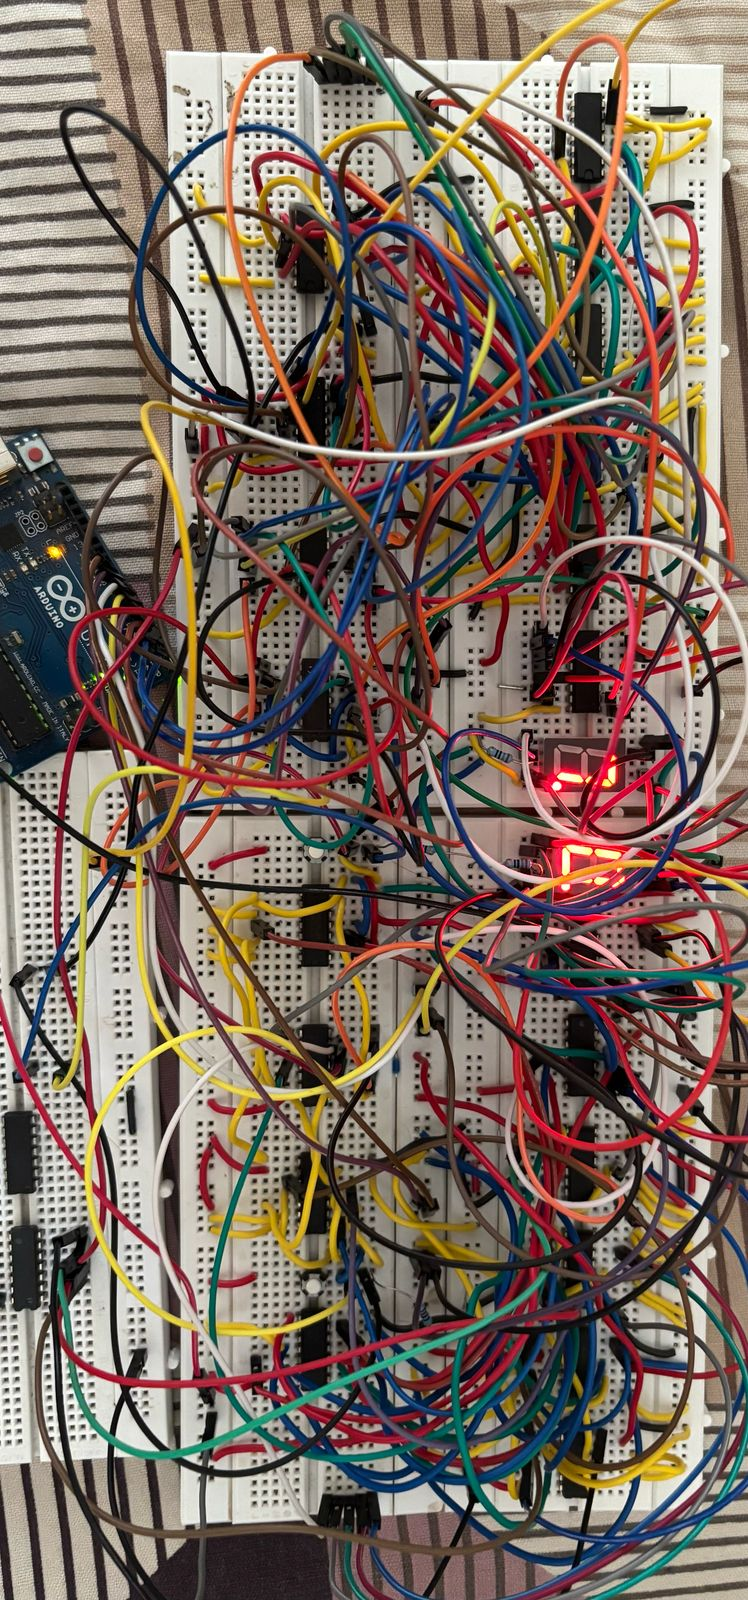
\includegraphics[width=0.5\linewidth]{figs/image-1.png}}
    \caption{Circuit}
    \label{fig:enter-label}
\end{figure}
The circuit may look daunting and complicated at first, let us break it down and study each module seperately.
\pagebreak
\subsection{Overview}
\begin{figure}[h!]
    \centering
    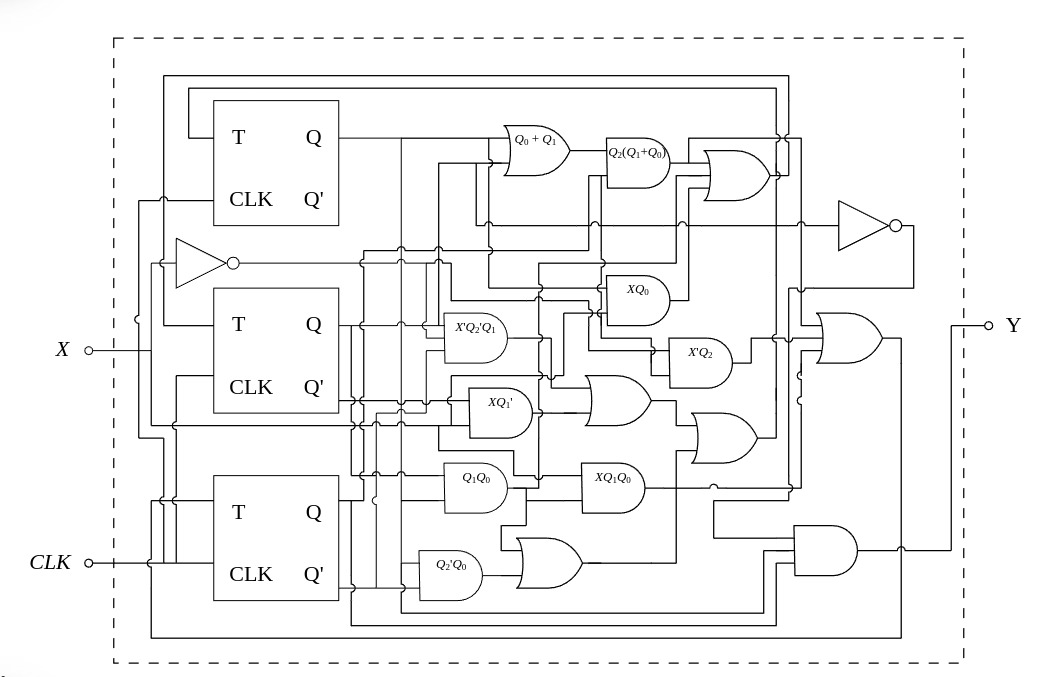
\includegraphics[width=1\linewidth]{figs/overview.png}
    \caption{Circuit Overview}
    \label{fig:enter-label}
\end{figure}
The upper part shows the units digit and the lower part shows the tens digit. For each digit, there is a module called $INC/DEC$ that either increments or decrements current count (by 1) depending on which button is pressed and returns the value to the $T$ of the flipflop (which becomes $Q$ of flipflop when clock becomes high). As for clock, logic is slightly different for each digit. For units place, output of the two button presses are ORed and given as clock (so that clock is only high when either button is pressed). For the tens place, each button press is first ANDed with either $\overline{Q_3}.\overline{Q_2}.\overline{Q_1}.\overline{Q_0}$ (decrement) or $Q_3\overline{Q_2}.\overline{Q_1}Q_0$ (increment) of units place and then ORed. This way clock is only high if incrementing button is pressed and units place is 9 or if decrementing button is pressed and units place is 0.

\subsection{JK to T Flip-Flop Conversion}
Since JK flip-flops were provided instead of T flip-flops, conversion was necessary. Converting a JK flip-flop to a T flip-flop can be done by simply shorting J and K ports of JK flip-flops.
\begin{displaymath}
\begin{array}{|c| c|c|c |c|}
\hline
T & Q_n & Q_{n+1} & J & K \\
\hline
0 & 0 & 0 & 0 & X \\
0 & 1 & 1 & X & 0 \\
1 & 0 & 1 & 1 & X \\
1 & 1 & 0 & X & 1 \\
\hline
\end{array}
\end{displaymath}
Writing Karnaugh-map for $J$
\begin{center}
\begin{karnaugh-map}[2][2][1][$Q_n$][$T$]
    \manualterms{0,X,1,X}
    \implicant{2}{3}
    %\implicant{5}{15}
    %\implicantedge{1}{3}{9}{11}
    %\implicantcorner
    %\implicantedge{4}{12}{6}{14}
\end{karnaugh-map}
\end{center}
We get,
\begin{align*}
    J = T
\end{align*}
Now writing karnaugh-map for $K$,
\begin{center}
\begin{karnaugh-map}[2][2][1][$Q_n$][$T$]
    \manualterms{X,0,X,1}
    \implicant{2}{3}
    %\implicant{5}{15}
    %\implicantedge{1}{3}{9}{11}
    %\implicantcorner
    %\implicantedge{4}{12}{6}{14}
\end{karnaugh-map}
\end{center}
We get,
\begin{align*}
    K = T
\end{align*}
\subsection{Changing Count}
\begin{figure}[h!]
    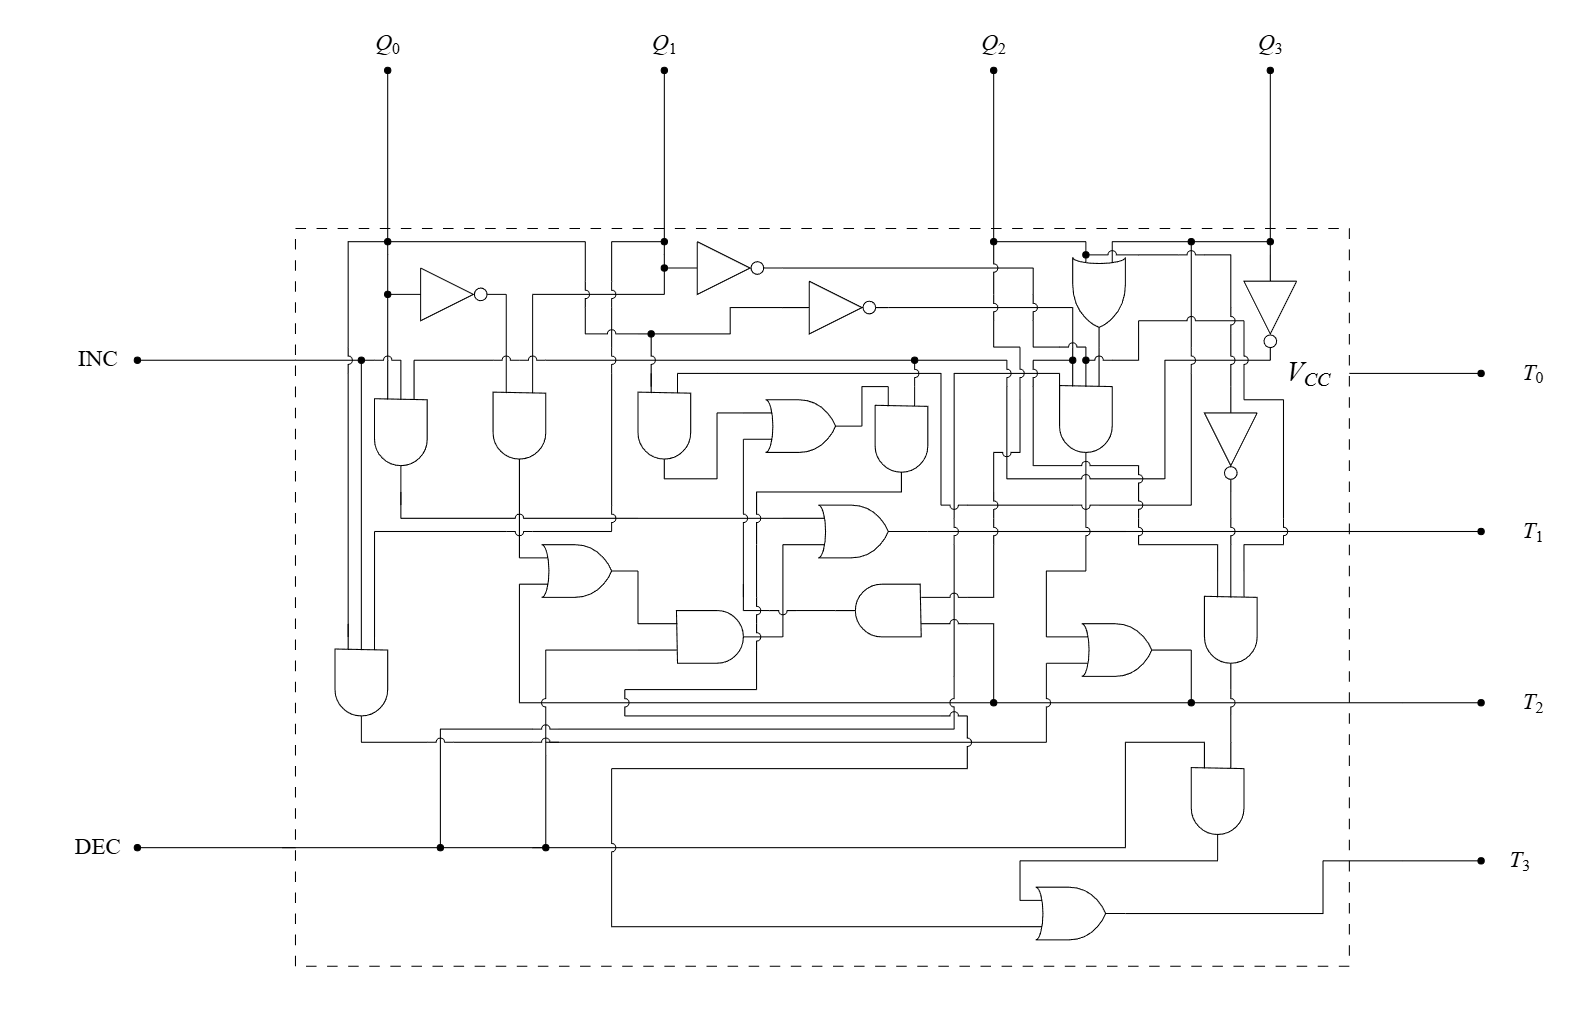
\includegraphics[width=1\linewidth]{figs/incdec.png}
    \caption{INC/DEC Module}
    \label{fig:enter-label}
\end{figure}
To either increment or decrement count depending on button press, we just AND the button press with their corresponding module (either increment or decrement) and OR the two outputs.
\subsection{Incrementing}
For the units digit in the UP counter, we derive the T flip-flop inputs using Karnaugh maps:
\pagebreak
\begin{table}[h!]
\centering
\begin{tabular}{|c|c|c|c|c|c|}
\hline
\textbf{Current State} & \textbf{$T_3$} & \textbf{$T_2$} & \textbf{$T_1$} & \textbf{$T_0$} & \textbf{Next State}\\
\hline
0000 & 0 & 0 & 0 & 1 & 0001 \\
0001 & 0 & 0 & 1 & 1 & 0010 \\
0010 & 0 & 0 & 0 & 1 & 0011 \\
0011 & 0 & 1 & 1 & 1 & 0100 \\
0100 & 0 & 0 & 0 & 1 & 0101 \\
0101 & 0 & 0 & 1 & 1 & 0110 \\
0110 & 0 & 0 & 0 & 1 & 0111 \\
0111 & 1 & 1 & 1 & 1 & 1000 \\
1000 & 0 & 0 & 0 & 1 & 1001 \\
1001 & 1 & 0 & 0 & 1 & 0000 \\
\hline
\end{tabular}
\end{table}
% Karnaugh map for T0
\begin{figure}[h!]
\centering
\begin{karnaugh-map}[4][4][1][$Q_1$,$Q_0$][$Q_3$,$Q_2$]
\manualterms{1,1,1,1,1,1,1,1,1,1,X,X,X,X,X,X}
\implicant{0}{10}
\end{karnaugh-map}
\caption{Karnaugh Map for $T_0$}
\end{figure}
\pagebreak
% Karnaugh map for T1
\begin{figure}[h!]
\centering
\begin{karnaugh-map}[4][4][1][$Q_1$,$Q_0$][$Q_3$,$Q_2$]
\manualterms{0,1,0,1,0,1,0,1,0,0,X,X,X,X,X,X}
\implicant{1}{7}
\end{karnaugh-map}
\caption{Karnaugh Map for $T_1$}
\end{figure}
% Karnaugh map for T2
\begin{figure}[h!]
\centering
\begin{karnaugh-map}[4][4][1][$Q_1$,$Q_0$][$Q_3$,$Q_2$]
\manualterms{0,0,0,1,0,0,0,1,0,0,X,X,X,X,X,X}
\implicant{3}{11}
\end{karnaugh-map}
\caption{Karnaugh Map for $T_2$}
\end{figure}
\pagebreak
% Karnaugh map for T3
\begin{figure}[h!]
\centering
\begin{karnaugh-map}[4][4][1][$Q_1$,$Q_0$][$Q_3$,$Q_2$]
\manualterms{0,0,0,0,0,0,0,1,0,1,X,X,X,X,X,X}
\implicant{7}{15}
\implicant{13}{11}
\end{karnaugh-map}
\caption{Karnaugh Map for $T_3$}
\end{figure}
\begin{align*}
&\text{From the Karnaugh map simplification, we derive:}\\
T_0 &= 1 \\
T_1 &= \overline{Q_3Q_0} \\
T_2 &= Q_1Q_0 \\
T_3 &= Q_3Q_0 + Q_2T_2
\end{align*}
\subsection{Decrementing}
Decrementing is done using Karnaugh Maps, 
\begin{table}[h!]
\centering
\begin{tabular}{|c|c|c|c|c|c|}
\hline
\textbf{Current State} & \textbf{$T_3$} & \textbf{$T_2$} & \textbf{$T_1$} & \textbf{$T_0$} & \textbf{Next State}\\
\hline
0000 & 1 & 0 & 0 & 1 & 1001 \\
0001 & 0 & 0 & 0 & 1 & 0000 \\
0010 & 0 & 0 & 1 & 1 & 0001 \\
0011 & 0 & 0 & 0 & 1 & 0010 \\
0100 & 0 & 1 & 1 & 1 & 0011 \\
0101 & 0 & 0 & 0 & 1 & 0100 \\
0110 & 0 & 0 & 1 & 1 & 0101 \\
0111 & 0 & 0 & 0 & 1 & 0110 \\
1000 & 1 & 1 & 1 & 1 & 0111 \\
1001 & 0 & 0 & 0 & 1 & 1000 \\
\hline
\end{tabular}
\end{table}
\pagebreak
% Karnaugh map for T0
\begin{figure}[h!]
\centering
\begin{karnaugh-map}[4][4][1][$Q_1$,$Q_0$][$Q_3$,$Q_2$]
\manualterms{1,1,1,1,1,1,1,1,1,1,X,X,X,X,X,X}
\implicant{0}{10}
\end{karnaugh-map}
\caption{Karnaugh Map for $T_0$}
\end{figure}
% Karnaugh map for T1
\begin{figure}[h!]
\centering
\begin{karnaugh-map}[4][4][1][$Q_1$,$Q_0$][$Q_3$,$Q_2$]
\manualterms{0,0,1,0,1,0,1,0,1,0,X,X,X,X,X,X}
\implicant{2}{10}
\implicantedge{4}{12}{6}{14}
\implicantedge{12}{8}{14}{10}
\end{karnaugh-map}
\caption{Karnaugh Map for $T_1$}
\end{figure}
\pagebreak
% Karnaugh map for T2
\begin{figure}[h!]
\centering
\begin{karnaugh-map}[4][4][1][$Q_1$,$Q_0$][$Q_3$,$Q_2$]
\manualterms{0,0,0,0,1,0,0,0,1,0,X,X,X,X,X,X}
\implicant{4}{12}
\implicant{12}{8}
\end{karnaugh-map}
\caption{Karnaugh Map for $T_2$}
\end{figure}
% Karnaugh map for T3
\begin{figure}[h!]
\centering
\begin{karnaugh-map}[4][4][1][$Q_1$,$Q_0$][$Q_3$,$Q_2$]
\manualterms{1,0,0,0,0,0,0,0,1,0,X,X,X,X,X,X}
\implicantedge{0}{0}{8}{8}
\end{karnaugh-map}
\caption{Karnaugh Map for $T_3$}
\end{figure}
\begin{align*}
&\text{From the Karnaugh map simplification, we derive:}\\
T_0 &= 1 \\
T_1 &= Q_1\overline{Q_0} + \overline{Q_1}.\overline{Q_0}.Q_2 + \overline{Q_1}.\overline{Q_0}.Q_3  \\
T_2 &= Q_2 .\overline{Q_1}.\overline{Q_0}  + Q_3.\overline{Q_1}.\overline{Q_0}  \\
T_3 &= \overline{Q_2}.\overline{Q_1}.\overline{Q_0}
\end{align*}
\subsection{Manual Reset Button}
A manual asynchronous reset button was added to reset count of number of people in the mess to $0$ regardless of current number of people in the mess. This was done by connecting all the $\overline{CLR}$ pins of the flip flops to a leg of the push button whose other end is grounded, and this leg of the push button is connected to $VCC$ through a pull up resistor.
\begin{figure}[h!]
\centering
\resizebox{0.2\textwidth}{!}{%
\begin{circuitikz}
\tikzstyle{every node}=[font=\large]
\draw (6.25,15.5) to[R] (6.25,13);
\draw (6.25,13) to[push button] (6.25,11.5);
\draw (6.25,11.5) to (6.25,11) node[ground]{};
\draw (6.25,13) to[short, -o] (7.5,13) ;
\draw (6.25,15.5) to[short, -o] (6.25,15.75) ;
\node [font=\large] at (6.25,16.25) {$VCC$};
\node [font=\large] at (6,10) {$GND$};
\node [font=\large] at (8.25,13) {$\overline{CLR}$};
\end{circuitikz}
}%

\label{fig:my_label}
\end{figure}
Through this process, we can ensure that $\overline{CLR}$ is always $HIGH$ unless button is pressed in which case $\overline{CLR}$ becomes $0$ which due to the design of the flipflop automatically nulls all outputs regardless of input.
\subsection{Clock}
The clock for the units digit is generated by ANDing the two button press signals. For the tens digit, the clock is generated by:
\begin{itemize}
\item ANDing the increment button with $Q_3\bar{Q_2}\bar{Q_1}Q_0$ of the units place (1 only when units digit is 9)
\item ANDing the decrement button with $\bar{Q_3}\bar{Q_2}\bar{Q_1}\bar{Q_0}$ of the units place (1 only when units digit is 0)
\item ORing the output of the two above mentioned AND gates.
\end{itemize}

\section{Results}
Images of circuits for some outputs,
\begin{figure}[h!]
    \centering
    \rotatebox{90}{
    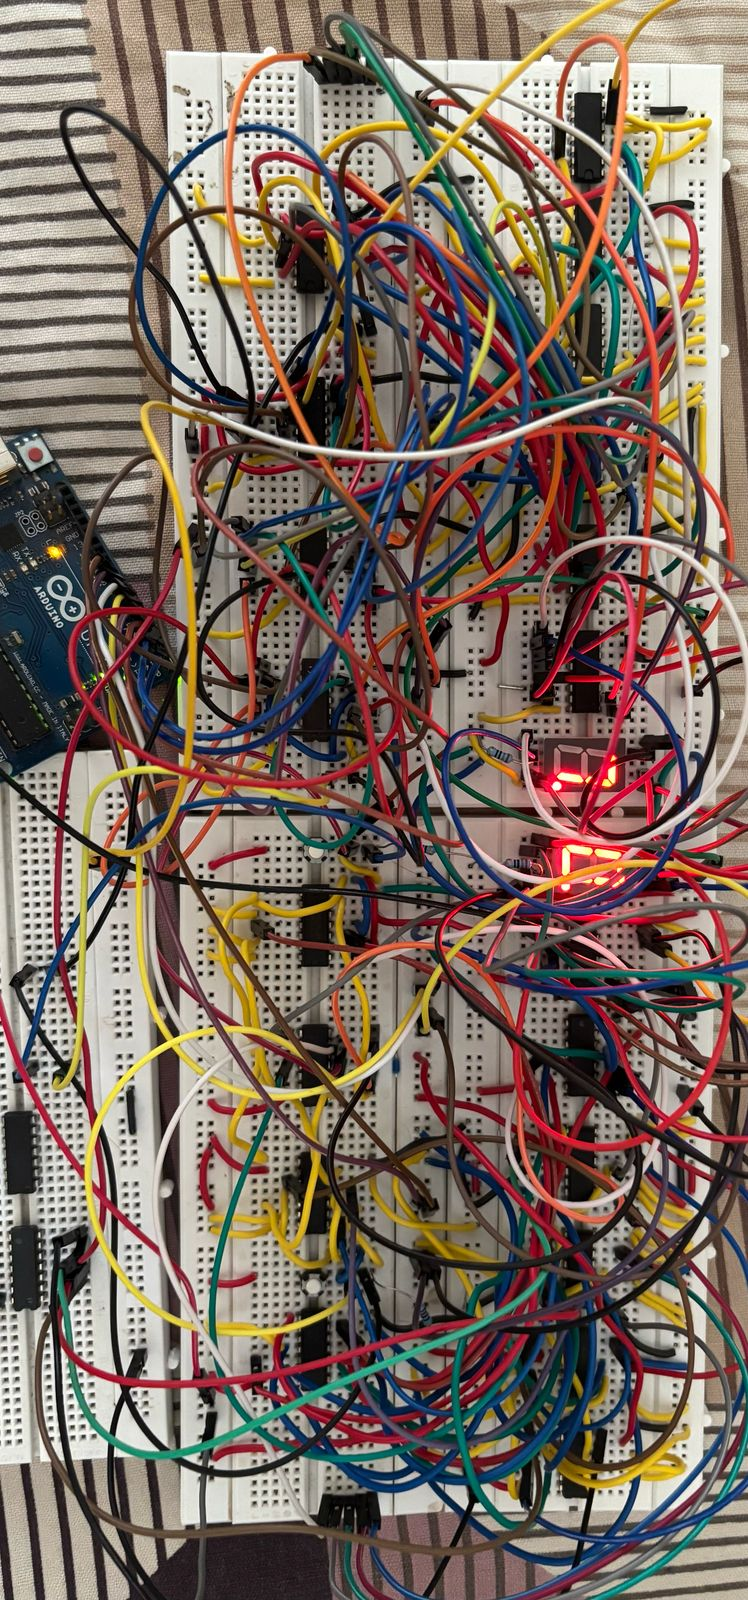
\includegraphics[width=0.5\linewidth]{figs/image-1.png}}
    \label{fig:enter-label}
\end{figure}
\pagebreak
\begin{figure}[h!]
    \centering
    \rotatebox{90}{
    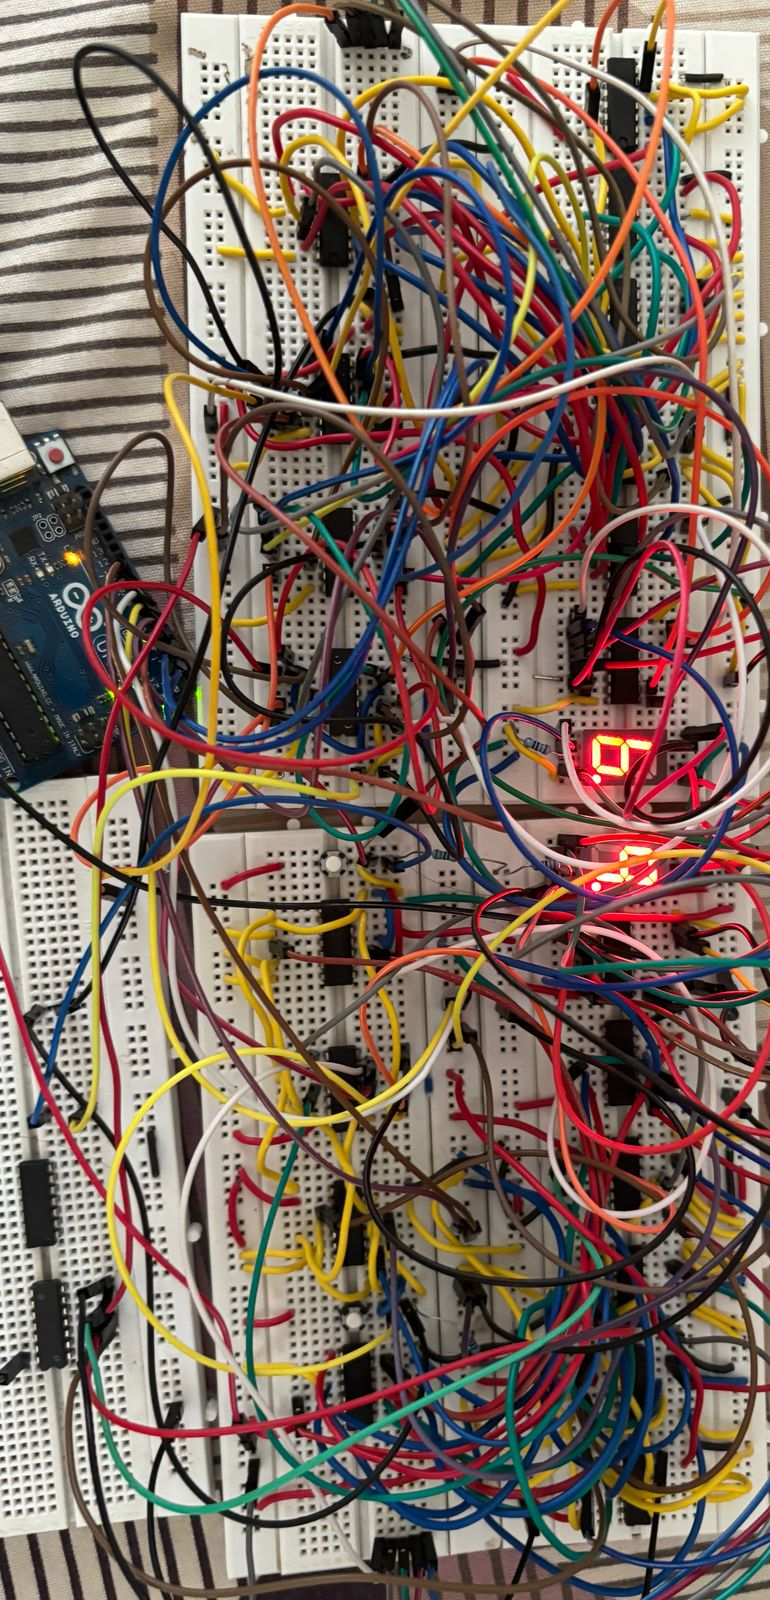
\includegraphics[width=0.5\linewidth]{figs/image-2.png}}
    \label{fig:enter-label}
\end{figure}
\begin{figure}[h!]
    \centering
    \rotatebox{90}{
    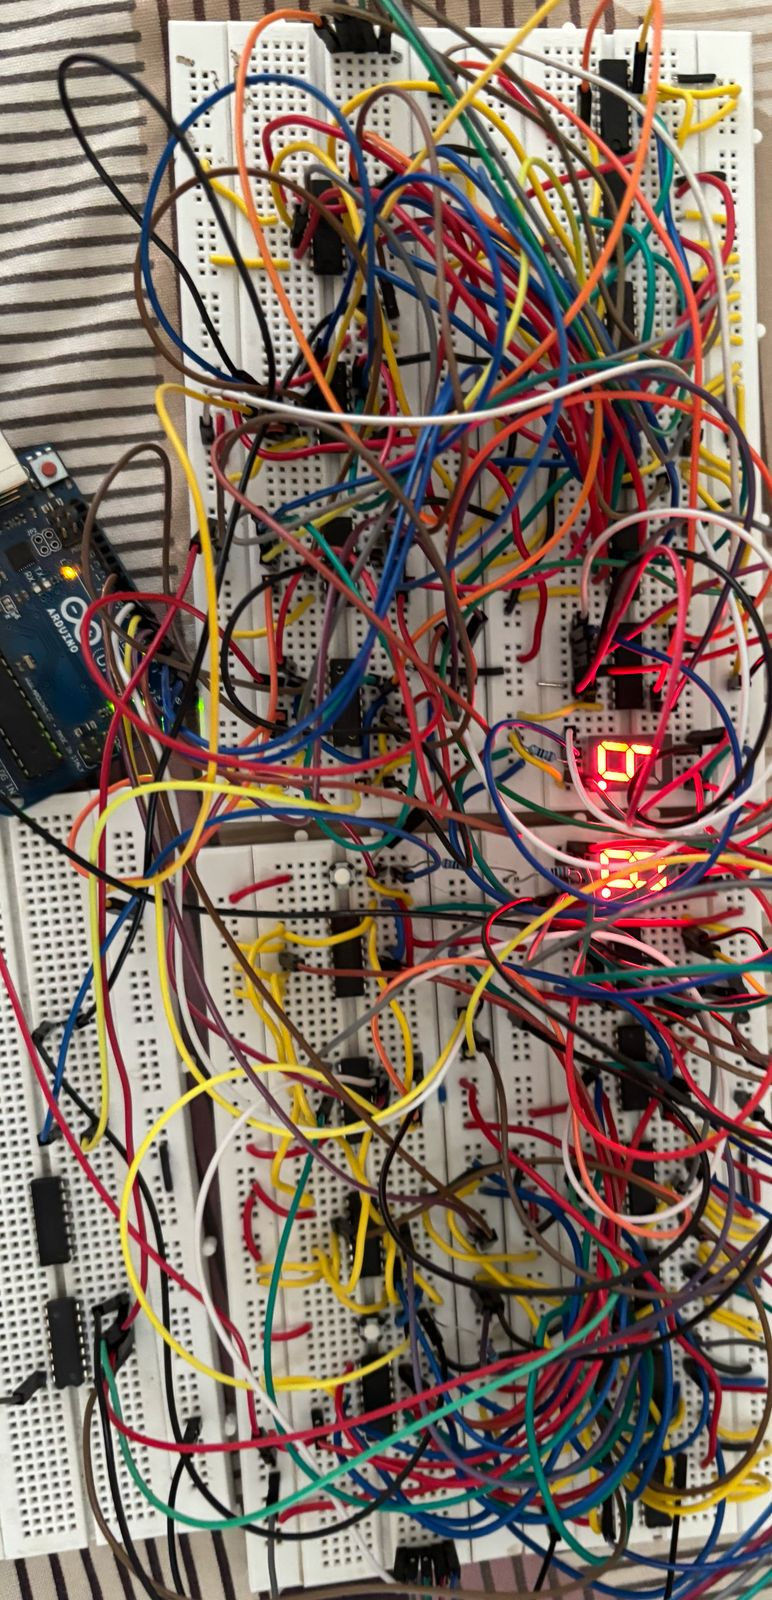
\includegraphics[width=0.5\linewidth]{figs/image-3.png}}
    \label{fig:enter-label}
\end{figure}
\pagebreak
\begin{figure}[h!]
    \centering
    \rotatebox{90}{
    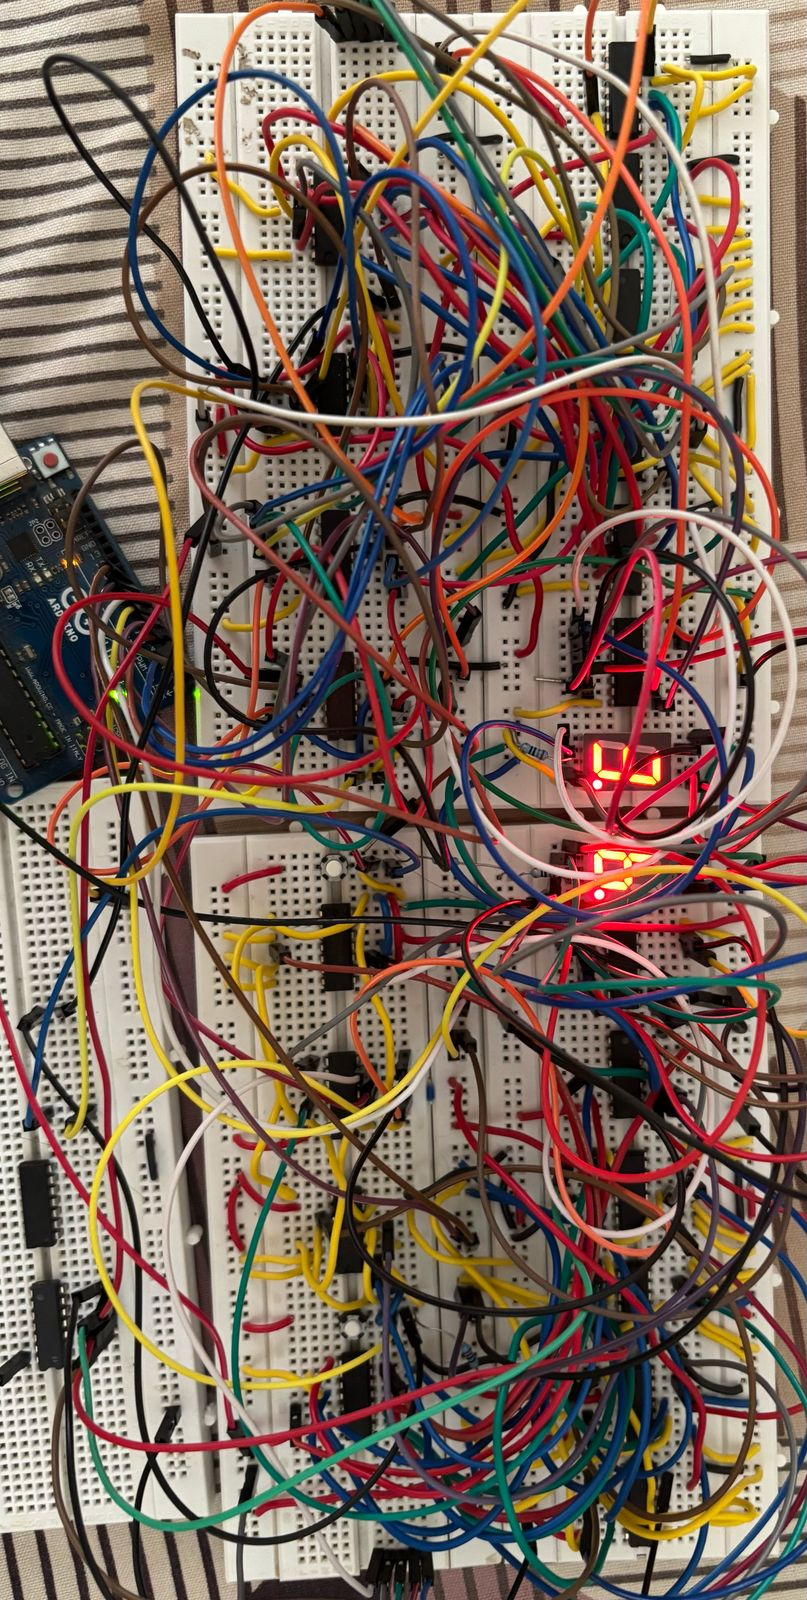
\includegraphics[width=0.5\linewidth]{figs/image-4.png}}
    \label{fig:enter-label}
\end{figure}
\begin{align*}
&\text{Videos of working may be found here,}\\ &\text{\url{https://github.com/ArjunPavanje/EE1200/tree/main/Experiment_8/vids}}
\end{align*}
\section{Conclusion}
The above report shows how a mess counter from 0-99 was built using Karnaugh Maps, multiplexing with a manual reset button.
\end{document}
